% !TEX program = xelatex
% !TeX encoding = utf8
% !TeX spellcheck = pl-PL

%%%%%%%%%%%%%%%%%%%%%%%%%%%%%%%%%%%%%%%%%%%%%%%%%%%%%%%%%%%%%%%%%%%%%%%%%%%
% Wybierz rodzaj pracy dyplomowej oraz wydział
% Pick thesis type and faculty
%%%%%%%%%%%%%%%%%%%%%%%%%%%%%%%%%%%%%%%%%%%%%%%%%%%%%%%%%%%%%%%%%%%%%%%%%%%
\documentclass[thesis=mgr,faculty=ee]{EE-dyplom} 

% thesis=[inz|mgr|bsc|msc]
%  * inz - praca inżynierska
%  * mgr - praca magisterska
%  * bsc - bachelor thesis
%  * msc - master thesis

% Skróty nazw wydziałów zgodne z domenami internetowymi
% Abbreviations of Faculties according to Internet subdomains
% faculty=[
%	arch,
%	gik,
%	ee,
%	wip
%	]

%%%%%%%%%%%%%%%%%%%%%%%%%%%%%%%%%%%%%%%%%%%%%%%%%%%%%%%%%%%%%%%%%%%%%%%%%%%
% Konfiguracja - do personalizacji
% Configuration - to be personalized
%%%%%%%%%%%%%%%%%%%%%%%%%%%%%%%%%%%%%%%%%%%%%%%%%%%%%%%%%%%%%%%%%%%%%%%%%%%
\instytut{Instytut Elektrotechniki Teoretycznej i Systemów Informacyjno-Pomiarowych}
\kierunek{Informatyka Stosowana}
\specjalnosc{Inżynieria Oprogramowania}
\title{Porównanie efektywności wybranych narzędzi służących do serwowania danych}
\engtitle{Comparison of the effectiveness of selected data serving tools}
\album{291089}
\author{inż. Jan Łukomski}
\promotor{prof. dr hab. inż. Remigiusz Rak}
\date{\the\year{}}
% \longdate{2077-07-27}

%\grantlicense{TRUE} % [TRUE|FALSE]

%%%%%%%%%%%%%%%%%%%%%%%%%%%%%%%%%%%%%%%%%%%%%%%%%%%%%%%%%%%%%%%%%%%%%%%%%%%
% Streszczenie pracy i abstract.
% In case of thesis in English swap the order - English version goes first.
%%%%%%%%%%%%%%%%%%%%%%%%%%%%%%%%%%%%%%%%%%%%%%%%%%%%%%%%%%%%%%%%%%%%%%%%%%%
\streszczeniepracy{
TODO na całą stronę

% \lipsum[1-4]
} % koniec streszczenia

\slowakluczowe{A, B, C}

\thesisabstract{
TODO

% \lipsum[1-4]
} % end of abstract

\thesiskeywords{X, Y, Z}

%%%%%%%%%%%%%%%%%%%%%%%%%%%%%%%%%%%%%%%%%%%%%%%%%%%%%%%%%%%%%%%%%%%%%%%%%%%
% Tu zaczyna się dokument
% Here is the beginning of the document
%%%%%%%%%%%%%%%%%%%%%%%%%%%%%%%%%%%%%%%%%%%%%%%%%%%%%%%%%%%%%%%%%%%%%%%%%%%
\begin{document}
    % Strony nagłówkowe
    % Headers
    \frontpages

    % Właściwa treść jest w pliku tekst/main.tex
    % Real contents is in tekst/main.tex
    % Rozdziały zaczynają się od "chapter"
\chapter{Wstęp}

Wybór technologii w ramach projektu jest decyzją strategiczną, którą nie jest łatwo zmienić na późniejszym etapie.
W celu utrzymywania produktu warto czasami podjąć trudną decyzję o zmodernizowaniu stosu techonologicznego.
Specyfika warunków oraz okoliczności tworzenia oprogramowania są kluczowymi elementami mającym bardzo duży wpływ na wybór technologii.
\section{Cel i zakres pracy}

Praca ta dokonuje analizy porównawczej trzech wybranych frameworków serwujących dane.
Pod uwagę został wzięty aspekt czasu odpowiedzi przy róznych warunkach.
Badanie ma na celu wskazać mocne oraz słabsze strony każdego z porównywanych narzędzi.
Badany jest wycinek rzeczywistości, którego istoną częścią jest różnica.
Bezwględne wartości mogą się różnić w zależności od warunków uruchomienia, natomiast relacje między badanymi obiektami powinny być stale zauważalne.


Testy można dzielić na rodzaje pod różnymi względami. Podstawowy podział testów został zaprezentowny na rysynku \ref{rys:test-types}\cite{atlassianRneRodzaje}.
\begin{figure}[!hb]
	\centering 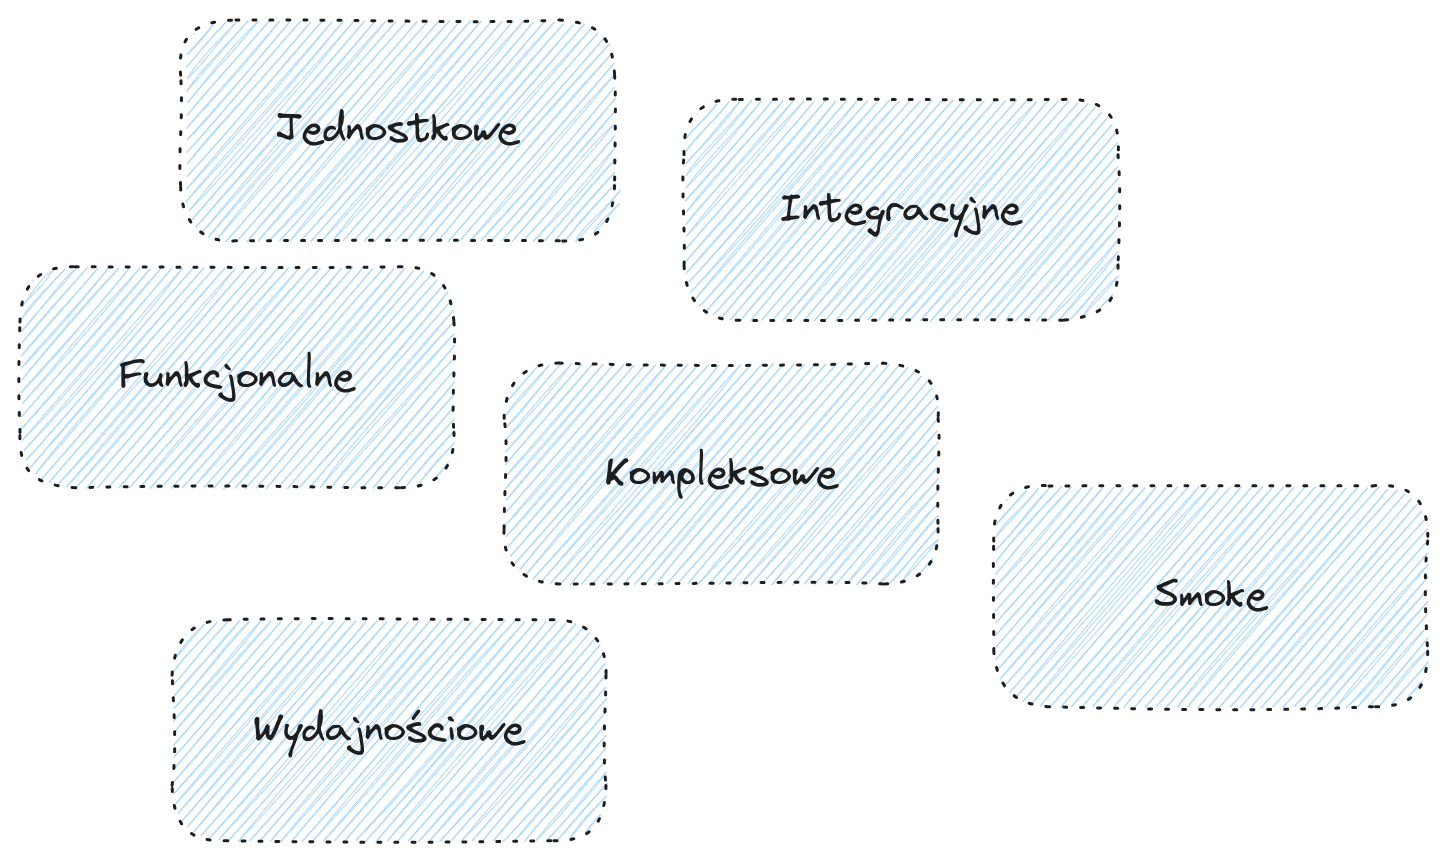
\includegraphics[width=1\linewidth]{rysunki/test-types.png}
	\caption{Rodzaje testów}
	\label{rys:test-types}
\end{figure}
Testy jednostkowe są testami pisanymi na stosunkowo niskim poziomie.
Nie jest jednoznacznie zdefiniowane czym jest jednostka która jest testowana.
Czasami jest to jedna funkcja, czasem jeden moduł.
Wszystko zależy od kontekstu badanego rozwiązania.
Charakteryzują się szybkością działania.
Nie jest potrzebna rozbudowana infrastruktura.
Dzięki temu można je uruchamiać często.

Kolejnymi testami na wyższym poziomie są testy integracyjne.
Badają one współdziałanie różnych modułów ze sobą. 
Do ich uruchomienia potrzebne jest zestawienie kilku modułów ze sobą więc wymagają one zazwyczaj większej infrastruktury niż testy jednostkowe.
Wiąże się to ograniczeniami związanymi ze zwiększonymi kosztami czasowymi oraz często powiązanymi z tym kosztami finansowymi.

Testy funkcjonalne nastawione są na sprawdzenie wymagań biznesowych aplikacji.
Ich złożoność podobna jest do testów integracyjnych.
Dziedziną badania jest sprawdzenie czy kluczowe elementy funkcjonalności są zrealizowane.

Kompleksowe testy badają całą aplikację.
Testy te wymagają postawienia całego systemu w celu jego przetestowania.
Z powodu ich kosztowności zaleca się ograniczenie ilości tych testów do minimalnej liczby.
Posiadanie ich najlepiej weryfikuje czy badana aplikacja działa.

Testy akceptacyjne weryfikują czy kluczowe wymagania biznesowe są zrealizowane.
Wymagają postawienia całej aplikacji przez co są kosztowne.

Smoke testy są istnym rodzajem testów bardzo łatwym w przeprowadzeniu.
Polegają na pobieżnym przejściu przez dowolny fragment systemu.
Jest to szybka weryfikacja czy podstawowy element systemu działa jak powinien.

Testy wydajnościowe sprawdzają czy w wymaganym obciążeniu aplikacja zachowuje się poprawnie.
Pomagaja znaleźć wąskie gardła systemu i zapobiec przerwie działania w przypadku wzrostu obsługiwanych użytkowników lub zwiększenia ilości przetważanych danych,

Wraz z wchodzeniem na wyższy poziom testowania koszty testów rosną \cite{testerzyPiramidaTestw}.
Stąd istnieje piramida testów prezentująca zaleźność liczby testów w zależności od rodzajów.
Piramida ta została zaprezentowana na rysunku \ref{rys:test-pyramid}.
\begin{figure}[!hb]
	\centering 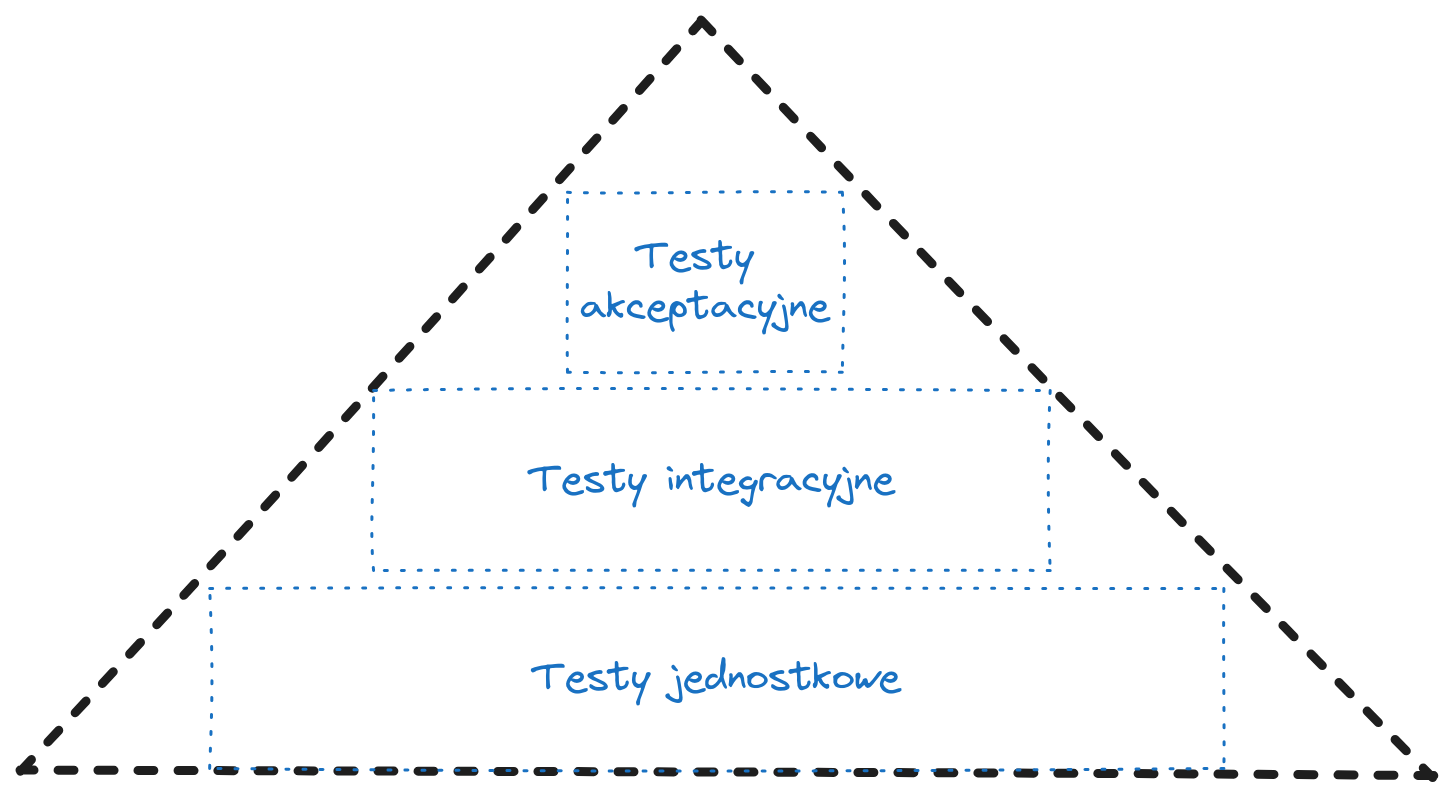
\includegraphics[width=1\linewidth]{rysunki/test-pyramid.png}
	\caption{Piramida testów}
	\label{rys:test-pyramid}
\end{figure}
Testy jednostkowe są na najniższym poziomie piramidy, a więc tego rodzaju testów powinno być najwięcej jako, że testy te są tanie w utrzymaniu.
Wraz z wzrostem wysokości piramidy, koszt utrzymania oraz uruchomienia testów rośnie.
Sposób podziału testów jest umowny więc wszystkie niewymienione rodzaje testów również znajdują się w piramidzie obok najbliższego rodzaju testów.


W niniejszej pracy testy przeprowadzone przynależą do kategorii testów wydajnościowych.
Są to kluczowe testy zapewniające o jednym z istotnych aspektów dobrze działającego oprogramowania.
Ich zadaniem jest identyfikacja obszarów ryzyka zachowania w czasie, wykorzystania zasobów oraz przepustowości \cite{testerzyTestowanieWydajnoci}.

\begin{figure}[!hb]
	\centering 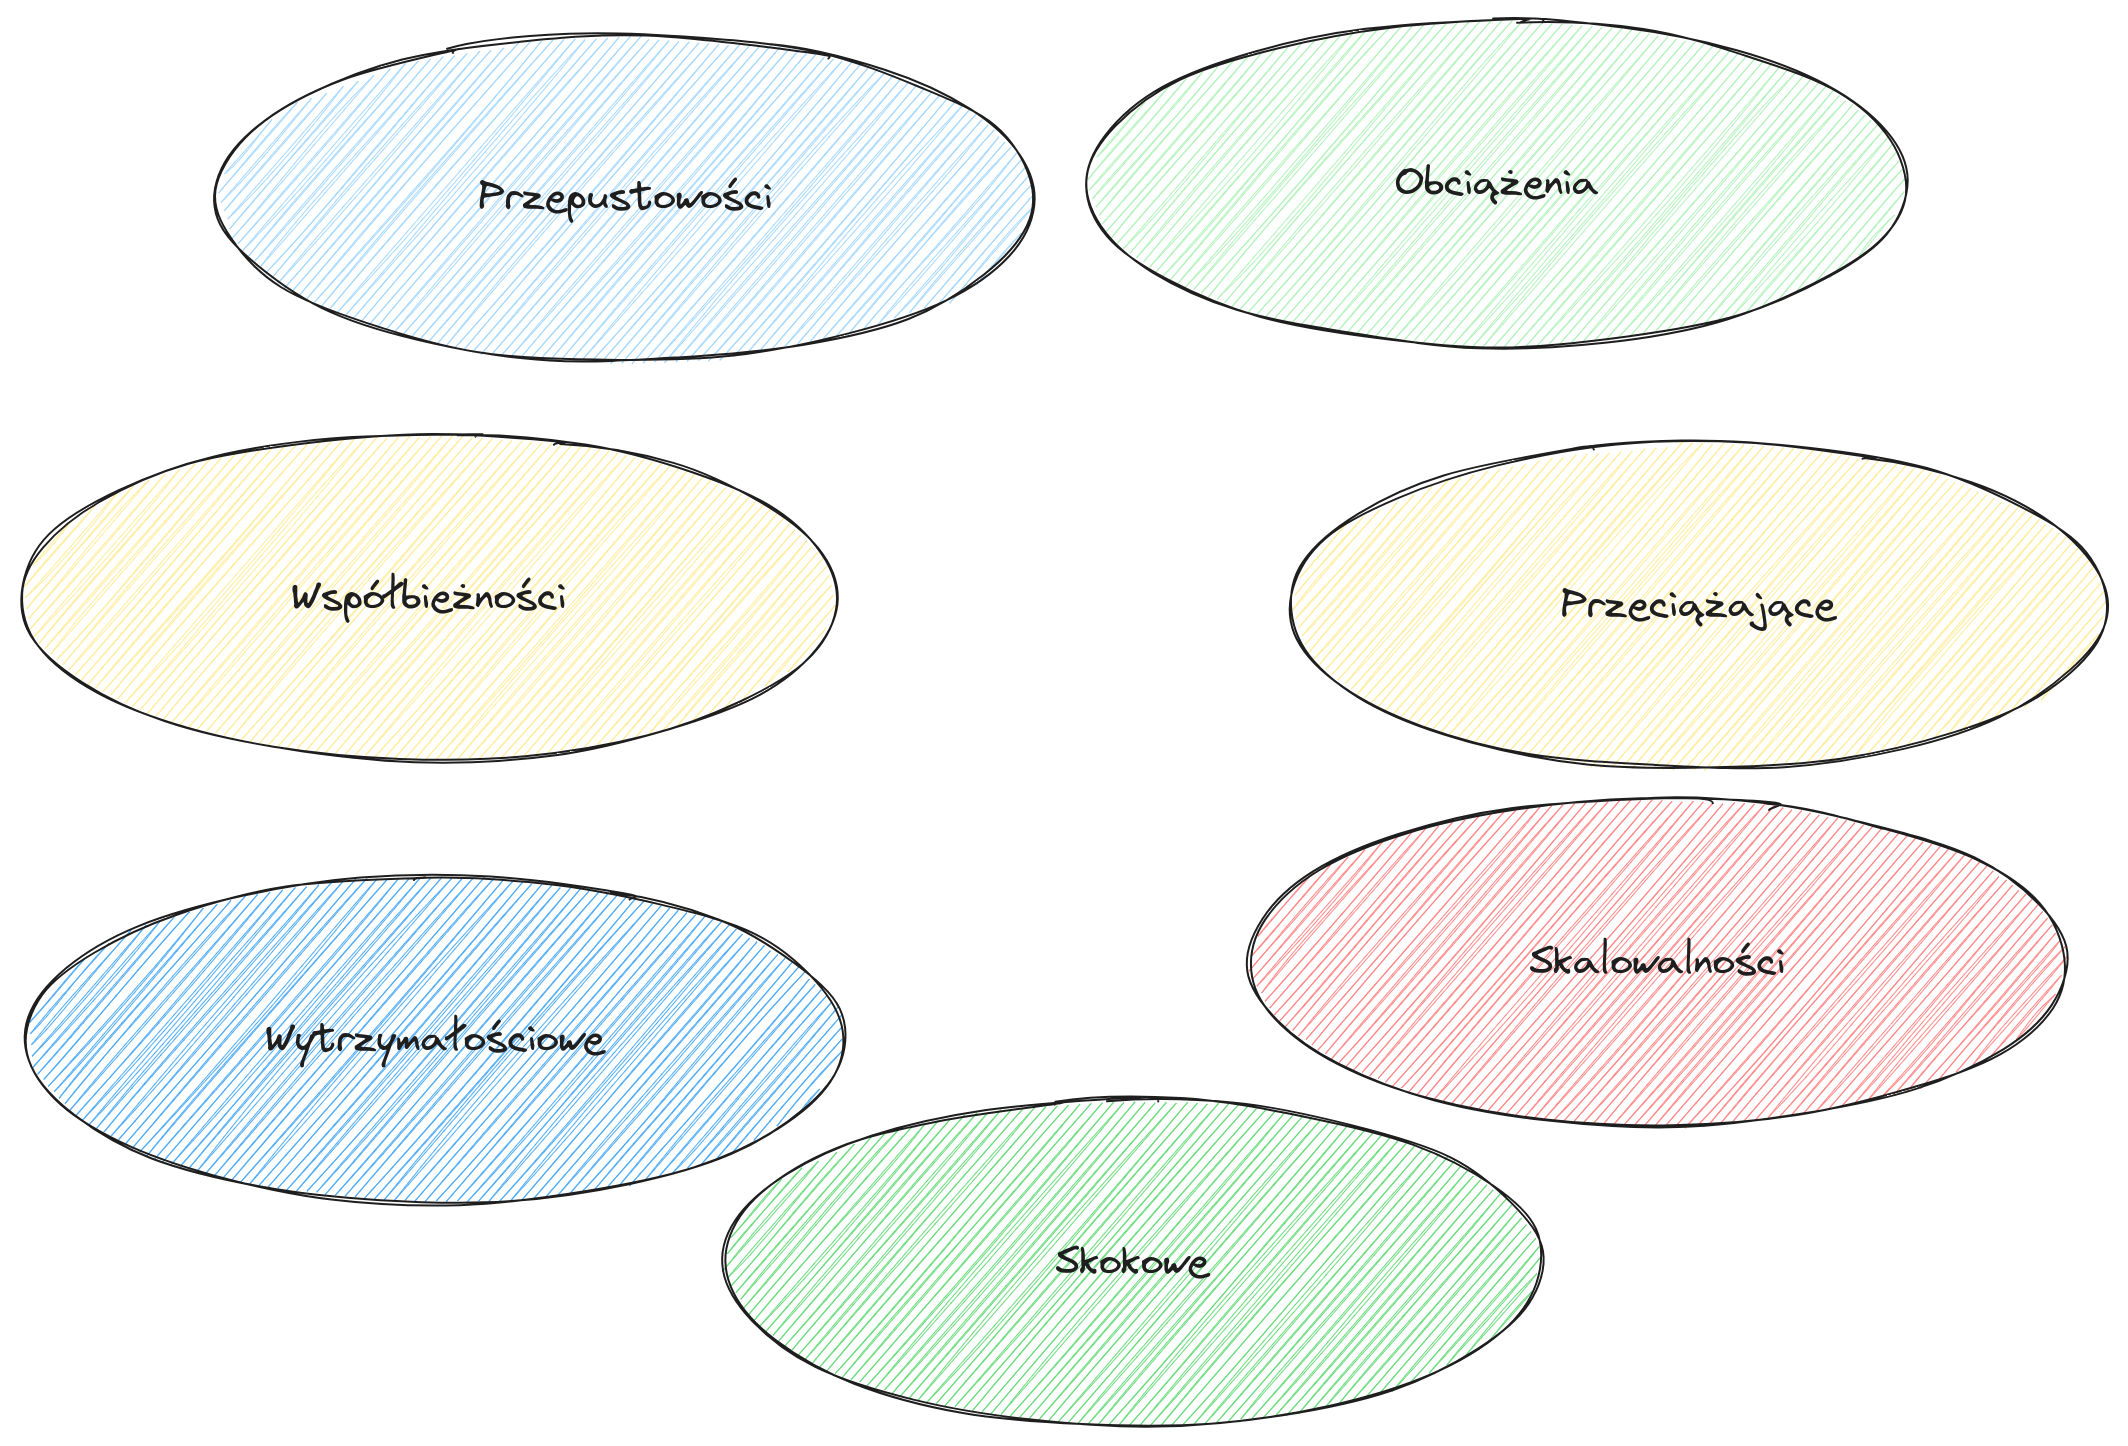
\includegraphics[width=1\linewidth]{rysunki/performance-tests.png}
	\caption{Typy testów wydajnościowych}
	\label{rys:performance-tests}
\end{figure}

Typy testów wydajnościowych zostały zaprezentowane na rysunku \ref{rys:performance-tests}.

Testowanie obciążenia to badanie zdolności systemu do obsługi wzrastającego obciążenia przy realistycznych, przywidywanych ilościach aktorów mających interakcje z systemem.

Testowanie przeciążające to badanie realizowane przy danych przekraczających realistyczne obciążenie. 
Ma ono na celu znalezienie granicy.

Testowanie skalowalności polega na zbadaniu granic funkcjonowania systemu przy zachowaniu większości pierwotnych założeń.
Pozwala ono na monitorowanie i wczesne reagowanie gdy nasz system wraz z rozwojem stopniowo przekracza wytyczone wymagania.

Testowanie skokowe bada reagowanie systemy na nagły, chwilowy wzrost obciążenia.
System powinien być w stanie wrócić no normalnego funkcjonowania, gdy obciążenie wróci do początkowego stanu.

Testowanie wytrzymałościowe skupia się na ocenie działania systemy w dłuższym okresie spracyficznym dla rozwiązania.
Skupia się na drobnych niedokładnościach, które wraz z czasem działania mogą urosnąć do rangi poważnych błędów.
Mogą to być błędy obliczeń związane z zaokrąglaniem lub wycieki pamięci.

Testowanie współbieżności sprawdza czy system działa poprawnie w przypadku przeprowadzania równoległych operacji.
Jestem to zazwyczaj trudny obszar do badania.

Testowanie przepustowości ocenia granice gdy system przestaje działać zgodnie z wymaganiami przy zwiekszonej liczbie aktorów mających interakcje z systemem.

Od innej strony można podzielić na testowanie statyczne oraz dynamiczne.
Testowanie statyczne wiąże się ze sprawdzeniem wymagań, architektury rozwiązania w celu znalezienia wąskiego gardła.
Czasami oznacza to również sprawdzenie używanych algorytmów.
Jest to bardzo ważna weryfikacja, ponieważ może zostać zrobiona w początkowej fazie projektu.
Poprawa problemu we wczesnej fazie zazwyczaj sprawia że jest on zdecydowanie mniej kosztowny.
Testowanie dynamiczne to testy jednostkowe, integracyjne, akceptacyjne, które zazwyczaj powstają wraz z rozwojem systemu.
Ich celem jest zwrócenie uwagi na problem niedostrzeżony w fazie testowania statycznego.


\chapter{Przegląd istniejących badań dla wybranych narzędzi}

\chapter{Opis koncepcji badania}

Badanie szeregowych zapytań zarówno dla zbioru FWB\_0 jak i FWB\_100K wskazało na Django jako framework wykazujący się kilku lub kilkunastokrotnie dłuższym czasem odpowiedzi.
Ponadto podczas bania limitu użytkowników wykazał się dużą odpornością na wzrost liczby użytkowników przy obsłudze większego zbioru danych.

W testach równoległych zapytań NestJS oraz .NET wypadają na podobnym poziomie z konsekwentną przewagą .NET.
NestJS wykazuje się kilkunastokrotnie wyższym limitem obsługiwanych użytkowników dla zwracanego zbioru FWB\_0.
Dla zbioru FWB\_100K nadal limit jest dwukrotnie wyższy od limitu .NET.

Nie da się wyodrębnić jednoznacznie zwycięzcę zestawienia.
Każdy framework wykazał się mocnymi stronami na tle innych w różnych kontekstach.

Wybór rozwiązania w projekcie zależy od wielu czynników, wśród których badane parametry są jednymi z wielu.
Niezwykle istotny jest czynnik ludzki w projekcie.
Osoby w projekcie kierują się różnymi motywacjami oraz mają doświadczenie z przeróżnymi narzędziami.
Zbadane obszary rzucają światło na fragment złożonego procesu decyzyjnego dotyczącego wyboru frameworka.
\section{Badanie pojedyńczego zapytania}
\section{Badania limitu użytkowników}

Kolejnym etapem badań było zbadanie granic ilości użytkowników, którymi wybrane narzędzia mogą obsłużyć równolegle.
Za kryterium niepowodzenia przyjęto sytuacje, w których narzędzie zwracało błąd lub nie udawało się uzyskać odpowiedzi w określonym czasie.
W celu określenia tych granic, przeprowadzono serię testów z różnymi liczbami użytkowników, wykorzystując metodę wyszukiwania binarnego.
Warto podkreślić, że uzyskane wyniki są przybliżone, ponieważ mogą nieco się różnić w zależności od warunków testowych.
Analiza granic jest kluczowa dla oceny skalowalności i wydajności badanych narzędzi w kontekście obsługi większej liczby użytkowników.
Otrzymane rezultaty pozwolają na lepsze zrozumienie możliwości i ograniczeń poszczególnych frameworków, co przyczynia się do bardziej świadomego wyboru technologii w projektach wymagających obsługi wielu użytkowników jednocześnie.

Analiza granic ilości użytkowników obsługiwanych równolegle przez badane narzędzia jest istotna z perspektywy projektowania i skalowania systemów, zwłaszcza w kontekście aplikacji o dużej liczbie użytkowników.
Poznanie tych granic pozwala na określenie optymalnej konfiguracji środowiska oraz planowanie zasobów potrzebnych do obsługi oczekiwanej liczby użytkowników.
Identyfikacja punktów granicznych umożliwia programistom dostosowanie strategii zarządzania obciążeniem oraz wprowadzenie optymalizacji w celu poprawy wydajności systemu.
Warto pamiętać, że wyniki tych testów mogą być podatne na zmiany w zależności od czynników zewnętrznych i warunków testowych.

\chapter{Opis wykorzystywanych narzędzi i bibliotek}

\section{Django}

Django to framework do tworzenia aplikacji insternetowych \cite{djangooverview}.
Jest to narzędzie, które nadaje się do szybkiego tworzenia zaawansowanych aplikacji internetowych, zachowując jednocześnie wysoką jakość i bezpieczeństwo kodu.
Jego popularność wynika z wielu czynników, w tym szybkości wdrażania projektów, bogatej palety wbudowanych funkcji oraz zabezpieczeń.

Jedną z głównych zalet Django jest jego zdolność do szybkiego rozwoju aplikacji od pomysłu do wdrożenia.
Framework ten oferuje wiele narzędzi i gotowych rozwiązań, które ułatwiają proces tworzenia stron internetowych, od autentykacji użytkowników po obsługę treści czy generowanie map strony.
Dzięki temu programiści mogą skupić się na kształtowaniu logiki aplikacji.
Posiada on wbudowane moduły, które pozwalają na szybki start projektu.
Są to mechanizmy obrony przed najczęstszymi atakami, takimi jak wstrzykiwanie SQL czy ataki typu cross-site scripting, czy system autentykacji użytkowników, zarządzanie kontami użytkowników oraz hasłami.

Django pozwala aplikacjom na elastyczne dostosowywanie się do zmieniających się wymagań i wzrostu liczby użytkowników.
Może być stosowany zarówno w małych projektach, jak i w dużych systemach obsługujących ogromne ruchy internetowe, co czyni go uniwersalnym narzędziem dla różnorodnych zastosowań.

Kod źródłowy frameworka Django jest udostępniony publicznie na zasadach otwartego oprogramowania.

\section{Dotnet}
\section{NestJS}
\section{K6}

Grafana k6 to narzędzie do testowania obciążenia aplikacji internetowych oraz wykonywania testów wydajnościowych \cite{grafanak6}.
Jest to część ekosystemu Grafana, znanej platformy do monitorowania i analizy danych, co zapewnia użytkownikom możliwość integracji testów wydajnościowych z analizą danych i wizualizacją wyników.

Jedną z kluczowych cech narzędzia Grafana k6 jest jego zdolność do symulowania zachowania użytkowników poprzez wysyłanie zapytań HTTP i analizowanie odpowiedzi serwera.
Można tworzyć zaawansowane scenariusze testowe, które odwzorowują różne zachowania użytkowników na stronie internetowej, takie jak logowanie, przeglądanie stron, czy też dodawanie produktów do koszyka.
Oferuje ono również bogate możliwości konfiguracyjne, które pozwalają dostosować testy do różnych scenariuszy.
Można określić warunki obciążeniowe, definiować progi wydajnościowe oraz zbierać szczegółowe dane diagnostyczne, które pomagają zidentyfikować przyczyny ewentualnych problemów.

Kod źródłowy k6 jest dostępny publicznie, co oznacza, że jest dostępny dla szerokiej społeczności deweloperów i testerów.
Dzięki temu można korzystać z bogatej dokumentacji, zgłaszać błędy oraz współpracować nad rozwojem narzędzia w ramach społeczności.

Grafana k6 to wszechstronne i potężne narzędzie do testowania wydajności aplikacji internetowych, które pozwala użytkownikom na symulowanie różnych scenariuszy obciążeniowych oraz monitorowanie wydajności.
Dzięki temu deweloperzy i testerzy mogą zapewnić, że ich aplikacje są wydajne i odpowiadają na oczekiwania użytkowników.
\section{Docker}

\chapter{Przygotowanie aplikacji}

Badanie szeregowych zapytań zarówno dla zbioru FWB\_0 jak i FWB\_100K wskazało na Django jako framework wykazujący się kilku lub kilkunastokrotnie dłuższym czasem odpowiedzi.
Ponadto podczas bania limitu użytkowników wykazał się dużą odpornością na wzrost liczby użytkowników przy obsłudze większego zbioru danych.

W testach równoległych zapytań NestJS oraz .NET wypadają na podobnym poziomie z konsekwentną przewagą .NET.
NestJS wykazuje się kilkunastokrotnie wyższym limitem obsługiwanych użytkowników dla zwracanego zbioru FWB\_0.
Dla zbioru FWB\_100K nadal limit jest dwukrotnie wyższy od limitu .NET.

Nie da się wyodrębnić jednoznacznie zwycięzcę zestawienia.
Każdy framework wykazał się mocnymi stronami na tle innych w różnych kontekstach.

Wybór rozwiązania w projekcie zależy od wielu czynników, wśród których badane parametry są jednymi z wielu.
Niezwykle istotny jest czynnik ludzki w projekcie.
Osoby w projekcie kierują się różnymi motywacjami oraz mają doświadczenie z przeróżnymi narzędziami.
Zbadane obszary rzucają światło na fragment złożonego procesu decyzyjnego dotyczącego wyboru frameworka.
\section{Zbiory danych}

W celu przeprowadzenia badania konieczne było przygotowanie odpowiednich zbiorów danych, które miały posłużyć do symulacji różnych scenariuszy.
W tym kontekście przygotowano dwa zbiory danych, aby umożliwić różnorodne analizy:

\begin{itemize}
  \item \textbf{FWB\_0} - Jest to zbiór pusty, pozbawiony jakichkolwiek elementów. Brak danych w tym zbiorze ma posłużyć do sprawdzenia zachowania systemu w sytuacji, gdy nie ma żadnych rekordów do przetworzenia.
  \item \textbf{FWB\_100K} - Ten zbiór składa się z 100 000 elementów. Każdy element tego zbioru reprezentuje pojedynczy rekord w bazie danych i zawiera unikalne identyfikatory (numery) oraz nazwy (tekstowe). Zbiór ten został przygotowany w celu przetestowania wydajności systemu oraz jego reakcji na duże ilości danych.
\end{itemize}
\phantom
\\
Jeden element to rekord w bazie danych zawierający ID (number) oraz nazwę (tekst).
Przygotowanie tych zbiorów danych stanowiło niezbędny krok przed przystąpieniem do właściwej analizy i symulacji różnych scenariuszy w badaniu. 
Dzięki tym zbiorom możliwe było zbadanie zachowania systemu w różnych warunkach oraz przeprowadzenie odpowiednich wniosków na podstawie uzyskanych wyników.

\chapter{Badanie aplikacji}

Badanie szeregowych zapytań zarówno dla zbioru FWB\_0 jak i FWB\_100K wskazało na Django jako framework wykazujący się kilku lub kilkunastokrotnie dłuższym czasem odpowiedzi.
Ponadto podczas bania limitu użytkowników wykazał się dużą odpornością na wzrost liczby użytkowników przy obsłudze większego zbioru danych.

W testach równoległych zapytań NestJS oraz .NET wypadają na podobnym poziomie z konsekwentną przewagą .NET.
NestJS wykazuje się kilkunastokrotnie wyższym limitem obsługiwanych użytkowników dla zwracanego zbioru FWB\_0.
Dla zbioru FWB\_100K nadal limit jest dwukrotnie wyższy od limitu .NET.

Nie da się wyodrębnić jednoznacznie zwycięzcę zestawienia.
Każdy framework wykazał się mocnymi stronami na tle innych w różnych kontekstach.

Wybór rozwiązania w projekcie zależy od wielu czynników, wśród których badane parametry są jednymi z wielu.
Niezwykle istotny jest czynnik ludzki w projekcie.
Osoby w projekcie kierują się różnymi motywacjami oraz mają doświadczenie z przeróżnymi narzędziami.
Zbadane obszary rzucają światło na fragment złożonego procesu decyzyjnego dotyczącego wyboru frameworka.

Badanie szeregowych zapytań zarówno dla zbioru FWB\_0 jak i FWB\_100K wskazało na Django jako framework wykazujący się kilku lub kilkunastokrotnie dłuższym czasem odpowiedzi.
Ponadto podczas bania limitu użytkowników wykazał się dużą odpornością na wzrost liczby użytkowników przy obsłudze większego zbioru danych.

W testach równoległych zapytań NestJS oraz .NET wypadają na podobnym poziomie z konsekwentną przewagą .NET.
NestJS wykazuje się kilkunastokrotnie wyższym limitem obsługiwanych użytkowników dla zwracanego zbioru FWB\_0.
Dla zbioru FWB\_100K nadal limit jest dwukrotnie wyższy od limitu .NET.

Nie da się wyodrębnić jednoznacznie zwycięzcę zestawienia.
Każdy framework wykazał się mocnymi stronami na tle innych w różnych kontekstach.

Wybór rozwiązania w projekcie zależy od wielu czynników, wśród których badane parametry są jednymi z wielu.
Niezwykle istotny jest czynnik ludzki w projekcie.
Osoby w projekcie kierują się różnymi motywacjami oraz mają doświadczenie z przeróżnymi narzędziami.
Zbadane obszary rzucają światło na fragment złożonego procesu decyzyjnego dotyczącego wyboru frameworka.

\chapter{Podsumowanie i wnioski}



    % Bibliografia - musi być
    % Bibliography - must exist
    \bibliografia

    % Strony końcowe - można zakomentować, jeśli zbędne
    % Additional pages - comment out if not needed
    
    % Wykaz symboli i skrótów - patrz opis w tekście przykładowym
    \acronymslist
    % Spis rysunków
    \listoffigures
    % Spis tabel
    \listoftables
    % Załączniki (plik appendices.tex)
    \easyappendices
\end{document}
%%%%%%%%%%%%%%%%%%%%%%%%%%%%%%%%%%%%%%%%%%%%%%%%%%%%%%%%%%%%%%%%%%%%%%%%%%%

